\input docmac

\title{Guide to Packaging with Descot}
\author{Shu Zhou and Aaron W. Hsu}
\contact{[shuzhou,awhsu]@indiana.edu}

\maketitlepage

\abstract
The Descot packager is designed to improve the portability of code that is distributed
by Scheme programmers. Rather than define code using a specific module system that must be individually translated, into either other module systems or into Descot metadata, the Descot packager provides an easy to write encoding of the core vocabulary in the Descot metalanguage in an extensible format. Instead of writing SRDF files for each file, you define a prelude file that defines some basic defaults for a set of files, and you then define specific properties for each specific library that you have defined. This forms, in effect,a module or package declaration of the file directly using Descot. The packager can then build an SRDF file suitable for uploading to a Descot server for publication and indexing, or it can be used to general system specific modules for use by the users of the code. 
\endabstract

\chapter{Program}{}%
For the first part Program, it contains two subparts. The first subpart is mainly about transformation from code to metadata and the second part is focused on metadata to code. 

\chapter{Package Organization}{}%

\section{Directory Layout}{}%
This is what we would do if we want to put a section in here. We could
also put something like the next in as well. This is what we would do if we want to put a section in here. We could
also put something like the next in as well. This is what we would do if we want to put a section in here. We could
also put something like the next in as well. This is what we would do if we want to put a section in here. We could
also put something like the next in as well. This is what we would do if we want to put a section in here. We could
also put something like the next in as well. This is what we would do if we want to put a section in here. We could
also put something like the next in as well. 

This is what we would do if we want to put a section in here. We could
also put something like the next in as well. This is what we would do if we want to put a section in here. We could
also put something like the next in as well. This is what we would do if we want to put a section in here. We could
also put something like the next in as well. This is what we would do if we want to put a section in here. We could
also put something like the next in as well. This is what we would do if we want to put a section in here. We could
also put something like the next in as well. This is what we would do if we want to put a section in here. We could
also put something like the next in as well. 

\section{Prelude}{}%

\section{library package}{}%

\chapter{Package Syntax}{}%

\chapter{RDF crash course}{}%

\medskip{\narrower\noindent
This is a quote from someone famous. This is a quote from someone
famous. This is a quote from someone famous. This is a quote from
someone famous. This is a quote from someone famous. This is a quote
from someone famous. This is a quote from someone famous. This is a
quote from someone famous.\par}\medskip

\noindent This is the next paragraph.

\medskip\verbatim
$ tex sample_doc.tex
  And it obeys indenting and ignores \funny things.
|endverbatim

\section{Subbed Section}{sec-sub-samp}%
\subsection{Real Subsection}{sub-sec-samp}%
This would contain the contents of the sub section.

You could also put a graphic somewhere in ehre.

\figplace{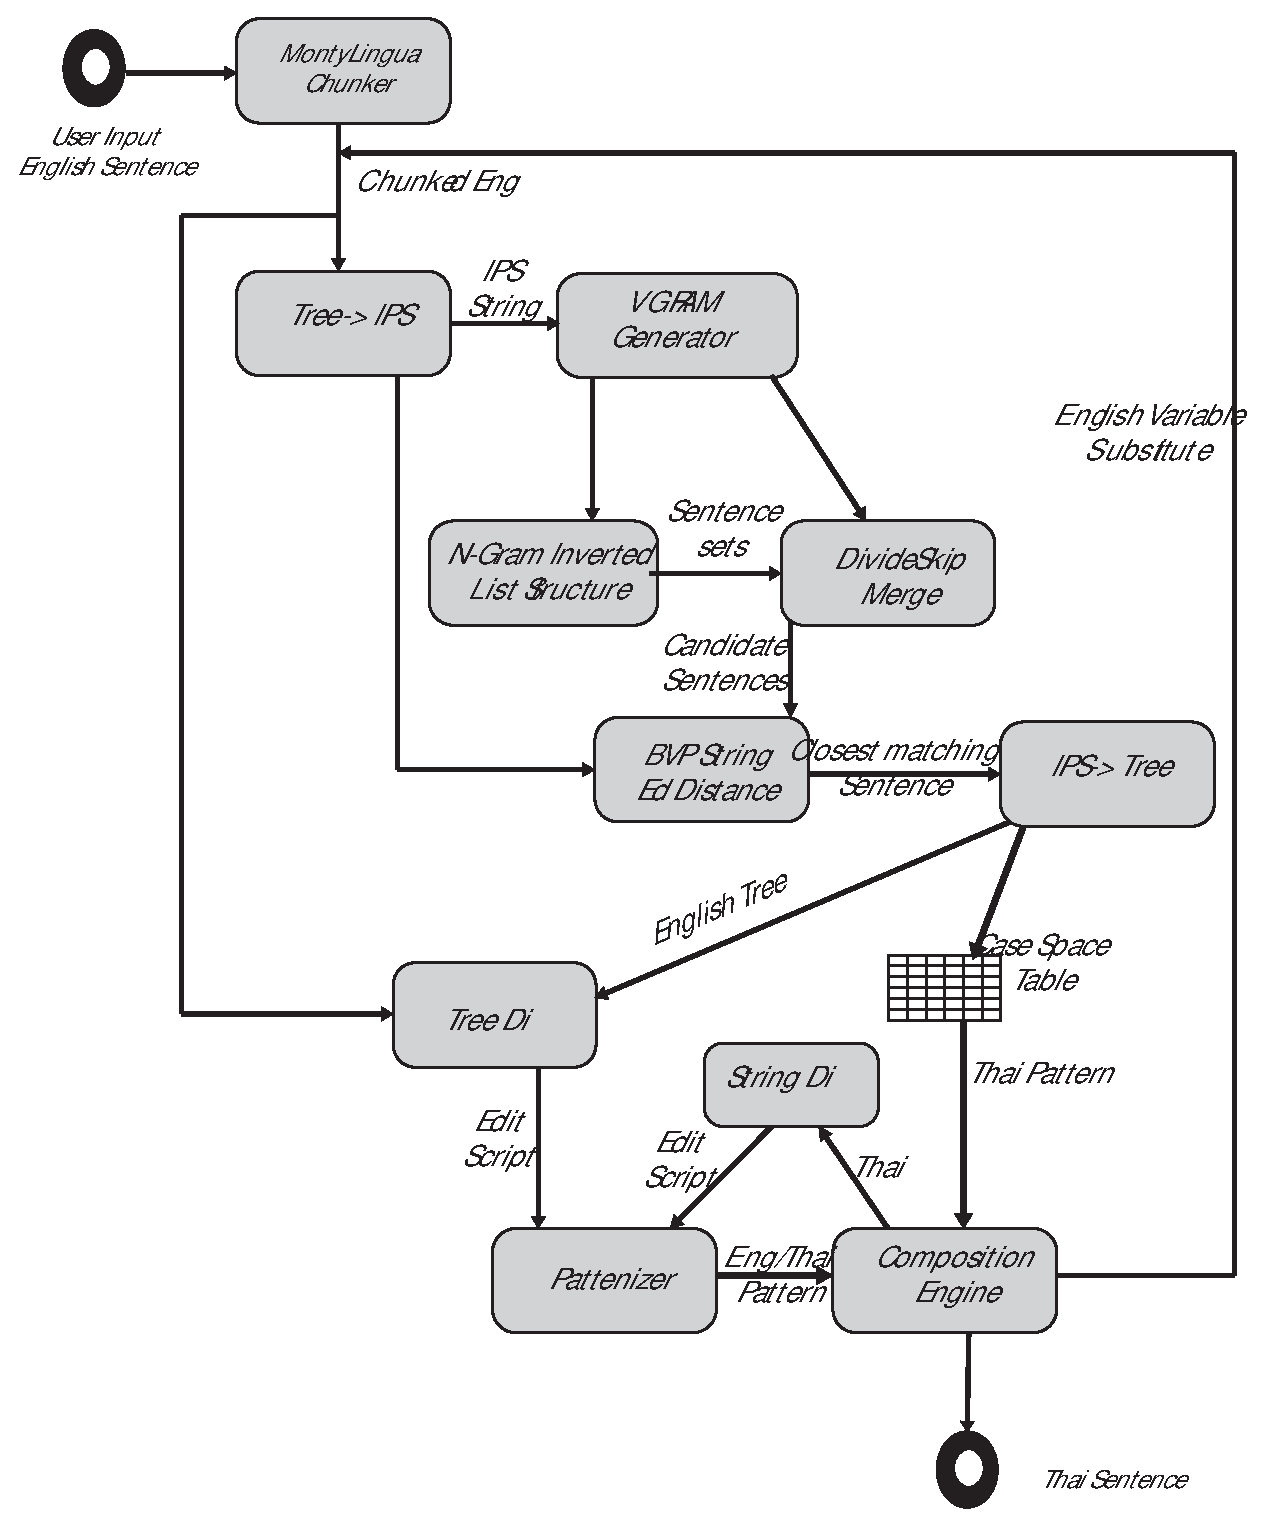
\includegraphics[width=15cm]{overview.eps}}
  {Workflow Outline}
  {Workflow Outline}

\bye
